% Chapter: Reinforcement Learning Algorithms
% Two sections: Classical Synthesis (Sutton-Baird), Deep Learning Era (Mnih-AlphaGo)

%%%%%%%%%%%%%%%%%%%%%%%%%%%%%%%%%%%%%%%%%%%%%%%%%%%%%%%%%%%%%%%%%%%%%%%%%%%%%%%
\subsection{The Classical Synthesis}
\label{sec:classical_synthesis}
%%%%%%%%%%%%%%%%%%%%%%%%%%%%%%%%%%%%%%%%%%%%%%%%%%%%%%%%%%%%%%%%%%%%%%%%%%%%%%%

\subsubsection{Monte Carlo Estimation}

When $P(s'|s,a)$ and $r(s,a)$ are unknown, the obvious approach is to use Monte Carlo (MC) to approximate them. These methods estimate value functions from sampled \textit{episodes} $(s_0, a_0, r_1, s_1, a_1, r_2, \ldots, s_T)$. The realized \textit{return} from state $s_t$ is
\begin{equation}
G_t = \sum_{k=0}^{T-t-1} \gamma^k r_{t+k+1}
\end{equation}
First-visit MC prediction averages $G_t$ over episodes for each state $s$, counting only its first occurrence per episode. Each first-visit return is an independent draw from the return distribution, so the sample mean converges almost surely to $V^\pi(s)$ by the strong law of large numbers \citep{sutton2018}. An incremental update is, $$V(s) \leftarrow V(s) + \alpha[G_t - V(s)]$$

For MC control, we can estimate action-values $Q(s,a)$ by averaging first-visit returns from each state-action pair, then improve the policy greedily: $\pi(s) = \argmax_a Q(s,a)$. Under exploring starts (every $(s,a)$ pair begins an episode infinitely often), this alternation converges to $Q^*$. \footnote{\citet{tsitsiklis2002} proved convergence even when the policy improves after every episode rather than waiting for complete evaluation. In practice, exploring starts is infeasible, so on-policy variants use $\varepsilon$-greedy exploration instead. These converge to $Q^*$ provided the exploration schedule satisfies the greedy-in-the-limit with infinite exploration (GLIE) condition: every state-action pair is visited infinitely often, and $\varepsilon_t \to 0$ so the policy converges to greedy in the limit.}

\subsubsection{Sutton (1988)}

Monte Carlo has two limitations. The agent must wait for episode termination to compute $G_t$, ruling out continuing tasks. And $G_t$ is unbiased ($\mathbb{E}[G_t \mid S_t = s] = V^\pi(s)$) but high-variance, because it sums random rewards over the entire \textit{trajectory}.

\citet{sutton1988} proposed temporal difference (TD) learning to fix both problems. TD(0) replaces the full return $G_t$ with a one-step target:
\begin{equation}
V(s_t) \leftarrow V(s_t) + \alpha \left[ r_{t+1} + \gamma V(s_{t+1}) - V(s_t) \right]
\end{equation}
The target $r_{t+1} + \gamma V(s_{t+1})$ depends on one random reward and one random transition, so its variance is low. The cost is bias. The bootstrap target $V(s_{t+1})$ is the agent's current estimate, not the true value. This is ``\textit{bootstrapping}''.\footnote{See Section~\ref{section:language} for the distinction between RL bootstrapping and Efron's resampling procedure.} As $V$ improves, the bias shrinks; the low variance persists regardless. Sutton demonstrated this tradeoff on a five-state random walk where TD(0) converged faster than Monte Carlo with less data.

The general TD($\lambda$) update interpolates between these extremes through an eligibility trace.\footnote{The eligibility trace records which states were recently visited, allowing credit assignment to propagate backward in time. States visited more recently receive stronger updates when the TD error is observed.}
\begin{equation}
V(s_t) \leftarrow V(s_t) + \alpha \, \delta_t \, e_t(s)
\end{equation}
where $\delta_t = r_{t+1} + \gamma V(s_{t+1}) - V(s_t)$ is the TD error and $e_t(s) = \gamma \lambda \, e_{t-1}(s) + \mathbbm{1}\{s = s_t\}$ is the eligibility trace for state $s$. Setting $\lambda = 0$ yields TD(0); setting $\lambda = 1$ recovers Monte Carlo returns. Intermediate $\lambda$ trades off variance against bias. \footnote{\citet{dayan1992} proved convergence of TD($\lambda$) for general $\lambda$ in the tabular case; \citet{jaakkola1994} gave a unified stochastic approximation proof covering both TD and Q-learning; \citet{tsitsiklis1997} extended the analysis to linear function approximation.}

\subsubsection{Watkins (1989)}

TD(0) learns value functions $V(s)$, but converting these to actions (the control problem) still requires knowing transition probabilities. Given $V(s')$ for all successor states, the agent needs to know which action leads to which successor. 

\citet{WatkinsDayan1992}, formalizing Watkins's 1989 PhD thesis, provided the solution. Instead of learning $V(s')$ learn $Q(s,a)$ (the action value function or the ``quality" of actions function) directly, the expected return from taking action $a$ in state $s$ and then behaving optimally. The optimal policy is then $\pi^*(s) = \argmax_a Q^*(s,a)$, requiring no model to act. The Bellman optimality equation provides the fixed-point condition:
\begin{equation}
Q^*(s,a) = \mathbb{E}\left[r + \gamma \max_{a'} Q^*(s',a') \mid s, a\right]
\end{equation}
Q-learning achieves this via the update
\begin{equation}
Q(s_t, a_t) \leftarrow Q(s_t, a_t) + \alpha \left[ r_{t+1} + \gamma \max_{a'} Q(s_{t+1}, a') - Q(s_t, a_t) \right]
\end{equation}
Q-learning converges to $Q^*$ under standard regularity conditions (Section~\ref{sec:stochastic_approx}). The maximization over $a'$ makes Q-learning \textit{off-policy}:\footnote{See Section~\ref{section:language} for the on-policy/off-policy distinction. Q-learning learns about the greedy policy $\pi^*(s) = \argmax_a Q(s,a)$ while collecting data with an exploratory policy. This exploratory policy needs only to be sufficiently ``exploratory'' and admits a wide range of policies; including a fully random policy.} the update target uses the greedy action at the next state regardless of the action actually taken. Therefore the agent can follow an $\varepsilon$-greedy exploration strategy or even a fully random policy, while learning about the optimal policy directly.

\subsubsection{Williams (1992)}

Value-based methods learn an action-value function and derive a policy from it. \citet{williams1992} derived an alternative, policy gradients, that optimize the policy directly by gradient ascent on expected return
\begin{equation}
\nabla_\theta J(\theta) = \mathbb{E}_{\pi_\theta} \left[ \sum_{t=0}^{T} \nabla_\theta \log \pi_\theta(a_t|s_t) \, G_t \right]
\end{equation}
where $G_t = \sum_{k=0}^{T-t} \gamma^k r_{t+k+1}$ is the discounted return from time $t$. The log-derivative trick allows the gradient to be estimated from sampled trajectories without differentiating through the environment dynamics.

Consider a robot arm that must apply a continuous torque $a \in \mathbb{R}$ to reach a target angle. Q-learning requires computing $\max_a Q(s,a)$ at every update, which becomes a nested optimization problem \footnote{In continuous action spaces, $\max_a Q(s,a)$ has no closed-form solution in general and must be solved numerically at every Bellman update. Discretizing a $d$-dimensional action space on a grid of $m$ points per dimension costs $O(m^d)$ evaluations per update step.} when the action space is continuous. A policy gradient method sidesteps the issue. Parameterize the policy as a Gaussian $\pi_\theta(a|s) = \mathcal{N}(\mu_\theta(s),\, \sigma_\theta^2(s))$,\footnote{The Gaussian distribution $\mathcal{N}(\mu, \sigma^2)$ has density $(2\pi\sigma^2)^{-1/2}\exp(-(a-\mu)^2/2\sigma^2)$. Here $\mu_\theta(s)$ and $\sigma_\theta(s)$ are neural network outputs parameterizing the policy mean and standard deviation.} sample an action, observe the return, and update $\theta$ by REINFORCE. Virtually all continuous-control results in reinforcement learning descend from the policy gradient framework for this reason.

%REINFORCE has a few practical issues, which motivated. First, because $G_t$ is a sum of stochastic rewards, gradient estimates can be noisy. Variance reduction techniques, including baselines $b(s_t)$ subtracted from $G_t$, are essential. One approach is to also estimate $V(s_t)$ and use it as a baseline. Secondly, REINFORCE uses each trajectory exactly once and discards it making it very sample-inefficient. This led to parallelization to gather more data faster and importance-sampling methods that re-use older data. Thirdly, a few outliers could destabilize learning if the gradient update is too severe. This led to KL trust regions and other limits on policy updates.  Thirdly, there is no mechanism to prevent the policy from collapsing into a deterministic policy early in training. This led to entropy regularization to encourage exploration by penalizing low-entropy policies.

\subsubsection{Tesauro (1994)}

\citet{tesauro1994}'s TD-Gammon demonstrated that temporal difference learning with neural network function approximation could achieve expert-level play in a domain with approximately $10^{20}$ legal positions\footnote{The state $\mathbf{x}(s)$ was a 198-dimensional binary encoding of the raw board (four units per board point per player indicating checker counts, plus bar and borne-off counts). The output was a four-component vector estimating probabilities of each game outcome (White/Black $\times$ normal win/gammon), and the move maximizing expected outcome among all legal moves was selected at each step.}. 

Backgammon was far beyond tabular methods, yet TD-Gammon trained a feedforward neural network to estimate the probability of winning from any board position. A hidden layer\footnote{A feedforward neural network stacks an input layer, one or more hidden layers, and an output layer; each unit in a hidden layer computes a weighted sum of its inputs and applies a nonlinear activation, here the logistic sigmoid $\sigma(x) = 1/(1+e^{-x})$, which maps any real number to $(0,1)$ and is identical to the binary logit link function.} of 80 sigmoid units fed a single sigmoid output.
\begin{equation}
\hat{V}(s) = \sigma\!\bigl(\mathbf{w}^\top \sigma(W\mathbf{x}(s) + \mathbf{b}) + c\bigr)
\end{equation}
where $\sigma$ is the logistic sigmoid, $W$ is the input-to-hidden weight matrix, and $\mathbf{w}$ is the hidden-to-output weight vector. The network was trained by self-play using TD($\lambda$) with $\lambda = 0.7$. After each move from position $s_t$ to $s_{t+1}$, the weights $\boldsymbol{\theta}$\footnote{$\boldsymbol{\theta}$ denotes the full vector of network weights and biases, generalizing the scalar $\theta$ used for policy parameters in earlier sections.} were updated by
\begin{equation}
\boldsymbol{\theta} \leftarrow \boldsymbol{\theta} + \alpha \bigl[\hat{V}(s_{t+1}) - \hat{V}(s_t)\bigr] \, \mathbf{e}_t
\end{equation}
where $\alpha$\footnote{The \emph{learning rate} $\alpha$ controls the step size of each parameter update. TD learning uses a semi-gradient step rather than true gradient descent, but $\alpha$ plays the same role: too large and updates overshoot; too small and convergence is slow.} is the step size, and the eligibility trace $\mathbf{e}_t = \sum_{k=1}^{t} \lambda^{t-k} \nabla_{\boldsymbol{\theta}} \hat{V}(s_k)$ accumulates exponentially decayed gradients of past predictions.\footnote{In the neural network case, the eligibility trace $\mathbf{e}_t \in \mathbb{R}^{|\boldsymbol{\theta}|}$ is a vector accumulating exponentially-weighted gradients, extending the scalar state-based trace to parameter space.} At game's end, $\hat{V}(s_{t+1})$ is replaced by the outcome $z \in \{0, 1\}$.

A single neural network $\hat{V}$ serves as the evaluation function for both players. At each turn, the current player selects the legal move maximizing $\hat{V}(s')$ from its own perspective. As the network improves, it generates stronger play on both sides, producing harder training games that drive further improvement. The dice rolls ensure diverse board positions without requiring an explicit exploration mechanism.\footnote{Version 2.1, trained on 1,500,000 games with 2-ply search, achieved near-parity with former world champion Bill Robertie and discovered novel positional strategies subsequently adopted by the human backgammon community.} 

\subsubsection{SARSA (1994)}

Q-learning learns the optimal action-value function regardless of the policy generating experience. This off-policy property is useful but introduces complications when combined with function approximation. \citet{rummery1994} introduced SARSA as an \textit{on-policy}\footnote{See Section~\ref{section:language} for the on-policy/off-policy distinction.} alternative that learns the value of the policy actually being followed. The name derives from the quintuple $(s_t, a_t, r_{t+1}, s_{t+1}, a_{t+1})$ used in each update:
\begin{equation}
Q(s_t, a_t) \leftarrow Q(s_t, a_t) + \alpha \left[ r_{t+1} + \gamma Q(s_{t+1}, a_{t+1}) - Q(s_t, a_t) \right]
\end{equation}
The key difference from Q-learning is that SARSA bootstraps from the action $a_{t+1}$ actually taken at the next state, rather than the greedy action $\argmax_{a'} Q(s_{t+1}, a')$. This makes the algorithm on-policy, since the target depends on the behavior policy generating the data.

If the agent follows an $\varepsilon$-greedy policy, SARSA converges to $Q^{\varepsilon\text{-greedy}}$, not $Q^*$\footnote{SARSA converges to $Q^*$ under GLIE (greedy in the limit with infinite exploration). A GLIE schedule explores all state-action pairs infinitely often but converges to the greedy policy asymptotically. The standard $\varepsilon$-greedy policy with $\varepsilon_t \to 0$ is one such schedule.} policies and standard step-size conditions (Section~\ref{sec:stochastic_approx}). This distinction matters when exploration is costly. Consider the cliff-walking problem, where an agent must traverse a gridworld with a cliff along one edge. The optimal path runs along the cliff edge (shortest route), but the $\varepsilon$-greedy policy occasionally falls off. Q-learning learns the optimal path because it evaluates the greedy policy; the agent falls off during learning but the Q-values reflect the optimal route. SARSA learns a safer path further from the cliff because it evaluates the actual exploratory policy; it accounts for the fact that exploration sometimes leads to catastrophic states. 

\subsubsection{Baird (1995)}

\citet{Baird1995} constructed a six-state star MDP demonstrating divergence of Q-learning with linear function approximation. The MDP has five outer states that all transition to a single inner state under the target policy. The off-policy behavior samples states uniformly. With linear function approximation, the weights grow without bound under repeated Q-learning updates. The source of instability is the interaction of three components, namely bootstrapping (updating from estimated values rather than observed returns), off-policy learning (training on data from a different policy than the target), and function approximation (representing the value function with a parameterized model). \citet{sutton2018} later named this the deadly triad. Any two components can be combined safely; all three together permit divergence. The mechanism underlying this instability is analyzed in Section~\ref{sec:deadly_triad}.

This result explains the asymmetry between Tesauro's success and Baird's failure. TD-Gammon used bootstrapping and function approximation but was on-policy, with training data coming from the same self-play policy whose value was being estimated. Baird's counterexample used all three components and diverged. Baird also proposed a constructive solution, namely residual gradient algorithms that perform gradient descent on the mean-squared Bellman residual, guaranteeing convergence at the cost of a different fixed point.

\subsubsection{Actor-Critic Methods (2000)}

The idea of maintaining both a policy (\textit{actor}) and a value function (\textit{critic}) dates to \citet{barto1983neuronlike}, who used a two-component system to solve the pole-balancing task. Actor-critic methods address the high variance of REINFORCE by replacing Monte Carlo returns with bootstrapped TD targets as the learning signal. The critic learns a value function $V(s)$ by TD updates.
\begin{equation}
V(s_t) \leftarrow V(s_t) + \alpha_c \, \delta_t, \quad \delta_t = r_{t+1} + \gamma V(s_{t+1}) - V(s_t)
\end{equation}
The actor updates the policy using the TD error as a sample of the advantage.
\begin{equation}
\theta \leftarrow \theta + \alpha_a \nabla_\theta \log \pi_\theta(a_t|s_t) \, \delta_t
\end{equation}
The TD error $\delta_t$ estimates $A^\pi(s_t, a_t) = Q^\pi(s_t, a_t) - V^\pi(s_t)$, the advantage of action $a_t$ over the average action.\footnote{That $\delta_t$ is an unbiased estimate of the advantage follows from the policy gradient theorem \citep{SuttonMcAllester2000}.} Positive advantages indicate the action was better than expected; negative advantages indicate it was worse.

\citet{konda2000} provided the first convergence proof for actor-critic algorithms with function approximation, showing convergence to a stationary point under two-timescale learning rates ($\alpha_c \gg \alpha_a$) and a compatibility condition on the critic architecture (Section~\ref{sec:actor_critic}).

%\citet{mnih2016a3c} introduced A3C (Asynchronous Advantage Actor-Critic), which parallelizes actor-critic across multiple CPU threads updating a shared parameter vector. Each thread runs its own copy of the environment, collects trajectories of length $t_{\max}$ or until a terminal state, computes gradients with respect to both actor and critic parameters, and applies updates asynchronously to the shared parameters without synchronization. The gradient for a trajectory $(s_0, a_0, r_0, \ldots, s_{t_{\max}})$ is accumulated by computing $n$-step returns $R_t = \sum_{k=0}^{n-1} \gamma^k r_{t+k} + \gamma^n V(s_{t+n})$ and using these as targets for both policy and value updates. The asynchrony provides implicit exploration, as different threads encounter different states, decorrelating the gradient updates. A3C achieved state-of-the-art results on Atari games while training in half the training time required by DQN on a GPU, using a single multi-core CPU, without the experience replay buffer required by DQN. The synchronous variant, A2C, collects batches from all workers before computing a single update; this sacrifices wall-clock speed for more stable gradients.

\subsubsection{Natural Policy Gradient (2001)}

Standard gradient descent treats all parameter directions equally, but policy parameters define probability distributions whose natural geometry is not Euclidean. \citet{Kakade2001} introduced the natural policy gradient, which measures progress in distribution space rather than parameter space. The update uses the Fisher information matrix $F(\theta)$:
\begin{equation}
F(\theta) = \mathbb{E}_{s \sim d^\pi, a \sim \pi_\theta} \left[ \nabla_\theta \log \pi_\theta(a|s) \nabla_\theta \log \pi_\theta(a|s)^\top \right]
\end{equation}
The natural gradient is
\begin{equation}
\tilde{\nabla}_\theta J(\theta) = F(\theta)^{-1} \nabla_\theta J(\theta)
\end{equation}
This direction is invariant to reparameterization of the policy. In the tabular softmax\footnote{The softmax function maps a vector $\mathbf{z}$ to a probability distribution: $\text{softmax}(z_i) = \exp(z_i)/\sum_j \exp(z_j)$. A softmax policy parameterizes action probabilities as $\pi_\theta(a|s) = \text{softmax}(\theta_{s,a})$.} case, a single natural gradient step with unit step size recovers one step of exact policy iteration (Section~\ref{sec:policy_gradient}).

The computational bottleneck is inverting $F(\theta) \in \mathbb{R}^{d \times d}$. Practical implementations use conjugate gradient methods to solve $F(\theta) x = \nabla_\theta J(\theta)$ without forming $F$ explicitly. This approach was later scaled to deep neural networks by TRPO and PPO.

\subsubsection{Fitted Value Iteration and Fitted Q-Iteration (2005)}
\label{sec:fvi_fqi_algorithms}

Tabular Q-learning maintains a separate entry for every state-action pair. When $|\mathcal{S}|$ is large or the state space is continuous, as in most applied problems, this is infeasible. \emph{Fitted Q-Iteration} (FQI) \citep{Ernst2005} replaces the tabular update with a supervised regression step: given a batch of transitions, fit a function approximator to the Bellman targets.

Let $\mathcal{F}$ be a function class mapping $\mathcal{S} \times \mathcal{A} \to \mathbb{R}$.\label{def:fqi} Initialize $Q_0 \equiv 0$. At each iteration $k = 0, 1, \ldots, K-1$: (i) draw $N$ transitions $(s_i, a_i, r_i, s_i')$ from a generative model; (ii) construct regression targets $y_i^{(k)} = r_i + \gamma \max_{a'} Q_k(s_i', a')$; (iii) set $Q_{k+1} \leftarrow \arg\min_{f \in \mathcal{F}} \frac{1}{N} \sum_{i=1}^N \bigl( f(s_i, a_i) - y_i^{(k)} \bigr)^2$. The output is the greedy policy $\pi_K(s) = \arg\max_a Q_K(s,a)$.

The regression step replaces the exact Bellman application with a projection onto $\mathcal{F}$: $Q_{k+1} = \Pi_{\mathcal{F}} \mathcal{T} Q_k$, where $\mathcal{T}$ is the Bellman optimality operator and $\Pi_{\mathcal{F}}$ is the $L^2$-projection under the sample distribution. Fitted Value Iteration (FVI) \citep{MunosSzepesvari2008} applies the same idea to the value function directly: $V_{k+1} = \Pi_{\mathcal{F}} \mathcal{T}^* V_k$, where $(\mathcal{T}^* V)(s) = \max_a \{ r(s,a) + \gamma \sum_{s'} P(s'|s,a) V(s') \}$.

With feature matrix $\Phi \in \mathbb{R}^{|\mathcal{S}| \times d}$ (rows $\phi(s)^\top$) and per-action weight vectors $\theta_a \in \mathbb{R}^d$, each FQI regression step for action $a$ reduces to the normal equations:
\begin{equation}
\theta_a^{(k+1)} = \bigl(\Phi^\top \Phi\bigr)^{-1} \Phi^\top y_a^{(k)},
\label{eq:fqi_normal}
\end{equation}
where $y_a^{(k)}(s) = r(s,a) + \gamma \sum_{s'} P(s'|s,a) \max_{a'} \phi(s')^\top \theta_{a'}^{(k)}$. Computation is $O(d^2 |\mathcal{S}| + d^3)$ per action per iteration. The FVI update takes the same form with a single weight vector $\theta_V$:
\begin{equation}
\theta_V^{(k+1)} = \bigl(\Phi^\top \Phi\bigr)^{-1} \Phi^\top V_{\mathrm{target}}^{(k)},
\label{eq:fvi_normal}
\end{equation}
where $V_{\mathrm{target}}^{(k)}(s) = \max_a \bigl\{ r(s,a) + \gamma \sum_{s'} P(s'|s,a) \phi(s')^\top \theta_V^{(k)} \bigr\}$. The finite-sample error theory for these methods is developed in Section~\ref{sec:fvi_fqi_theory}.

%%%%%%%%%%%%%%%%%%%%%%%%%%%%%%%%%%%%%%%%%%%%%%%%%%%%%%%%%%%%%%%%%%%%%%%%%%%%%%%
\subsection{The Deep Learning Era}
%%%%%%%%%%%%%%%%%%%%%%%%%%%%%%%%%%%%%%%%%%%%%%%%%%%%%%%%%%%%%%%%%%%%%%%%%%%%%%%

\subsubsection{Deep Q-Networks (2015)}

\citet{mnih2015} trained a single convolutional neural network\footnote{A convolutional neural network applies learned spatial filters to detect local patterns in grid-structured data, commonly used for image inputs.} to play 49 Atari 2600 games directly from pixel inputs ($210 \times 160 \times 3$) and a scalar score, using no game-specific features.

The architecture processed four consecutive frames through three convolutional layers and a fully connected layer.\footnote{A fully connected layer computes $y = Wx + b$ where every input unit is connected to every output unit with learned weights $W$ and biases $b$; it is the affine transformation familiar from linear regression, followed by a nonlinear activation.} The network $Q(s, a; \theta)$ was trained to minimize the squared temporal difference error
\begin{equation}
L(\theta) = \mathbb{E}_{(s,a,r,s') \sim \mathcal{D}} \left[ \left( r + \gamma \max_{a'} Q(s', a'; \theta^-) - Q(s, a; \theta) \right)^2 \right]
\end{equation}

Two innovations stabilized learning. \textit{Experience replay} \citep{Lin1992} stored transitions $(s, a, r, s')$ in a buffer $\mathcal{D}$ and sampled uniformly for training, breaking the temporal correlation between consecutive updates. A \textit{target network} used a frozen copy of parameters $\theta^-$, updated periodically,\footnote{The buffer held $10^6$ transitions; the target network $\theta^-$ was synchronized to $\theta$ every $C = 10{,}000$ steps.} so the regression target does not shift with each gradient step.

%These techniques address the deadly triad identified by Baird. Experience replay creates a more stationary data distribution, partially mitigating off-policy issues. The target network holds the bootstrap target fixed between updates, making the regression problem approximately stationary. Neither technique provides theoretical guarantees, but the empirical success demonstrated that the deadly triad can be managed in practice.

DQN exceeded human-level performance on 29 of 49 games using a single architecture and hyperparameters.\footnote{\emph{Hyperparameters} are design choices fixed before training begins, such as network depth, learning rate, and replay buffer size; they are not estimated by gradient descent.} Games requiring long-horizon planning or sparse rewards, such as Montezuma's Revenge, remained difficult.

\subsubsection{TRPO and PPO (2015, 2017)}

Policy gradient methods suffer from a practical instability: a single large gradient step can move the policy into a region where performance collapses and recovery is slow.

\citet{Schulman2015} addressed this with Trust Region Policy Optimization (TRPO). TRPO solves the constrained optimization problem
\begin{equation}
\max_\theta \; L_{\theta_{\text{old}}}(\theta) \quad \text{subject to} \quad \bar{D}_{\mathrm{KL}}(\theta_{\text{old}}, \theta) \leq \delta
\end{equation}
where $L$ is a surrogate objective based on the advantage function $A^\pi(s,a) = Q^\pi(s,a) - V^\pi(s)$.\footnote{The Kullback-Leibler divergence $D_{\mathrm{KL}}(p \| q) = \sum_x p(x) \log(p(x)/q(x))$ measures statistical distance between distributions. The bar denotes expectation over states: $\bar{D}_{\mathrm{KL}} = \mathbb{E}_{s}[D_{\mathrm{KL}}(\pi_{\theta_{\text{old}}}(\cdot|s) \| \pi_\theta(\cdot|s))]$.}

\citet{Schulman2017} proposed Proximal Policy Optimization (PPO) as a simpler alternative. PPO replaces the KL constraint with a clipped surrogate objective:
\begin{equation}
L^{\text{CLIP}}(\theta) = \mathbb{E}_t \left[ \min\!\left( r_t(\theta) \hat{A}_t, \; \text{clip}(r_t(\theta), 1-\varepsilon, 1+\varepsilon) \hat{A}_t \right) \right]
\end{equation}
where $r_t(\theta) = \pi_\theta(a_t|s_t) / \pi_{\theta_{\text{old}}}(a_t|s_t)$ is the probability ratio. The clipping removes the incentive for $r_t(\theta)$ to move outside the interval $[1-\varepsilon, 1+\varepsilon]$, penalizing large policy updates without explicitly computing a divergence measure.

PPO outperformed A2C, TRPO, and the cross-entropy method on continuous control benchmarks and achieved the highest average reward on 30 of 49 Atari games among the methods tested. PPO became the default policy optimization algorithm for large-scale RL applications, demonstrating that constraining the magnitude of policy updates is essential for stable optimization.

\subsubsection{Soft Actor-Critic (2018)}

\citet{Haarnoja2018} introduced Soft Actor-Critic (SAC), which adds entropy regularization to the actor-critic framework. The agent maximizes expected return plus an entropy bonus:
\begin{equation}
J(\theta) = \mathbb{E}_{\pi_\theta}\left[\sum_{t=0}^\infty \gamma^t \left(r_t + \tau \mathcal{H}(\pi_\theta(\cdot|s_t))\right)\right]
\end{equation}
where $\mathcal{H}(\pi) = -\sum_a \pi(a) \log \pi(a)$ is the entropy and $\tau > 0$ is a temperature parameter. The entropy bonus encourages exploration by penalizing deterministic policies. The optimal policy under this objective is softmax in the Q-values: $\pi^*(a|s) \propto \exp(Q^*(s,a)/\tau)$, connecting to discrete choice models in econometrics.

SAC maintains two Q-networks (to reduce overestimation bias) and a policy network. The soft Bellman operator for the critic is:
\begin{equation}
(T^\pi Q)(s,a) = r(s,a) + \gamma \mathbb{E}_{s'}\left[ V(s') \right], \quad V(s) = \mathbb{E}_{a \sim \pi}[Q(s,a) - \tau \log \pi(a|s)]
\end{equation}
SAC is off-policy (using experience replay), handles continuous actions naturally, and achieves state-of-the-art sample efficiency on continuous control benchmarks. The entropy regularization provides automatic exploration without $\varepsilon$-greedy schedules.

\begin{figure}[t]
\centering
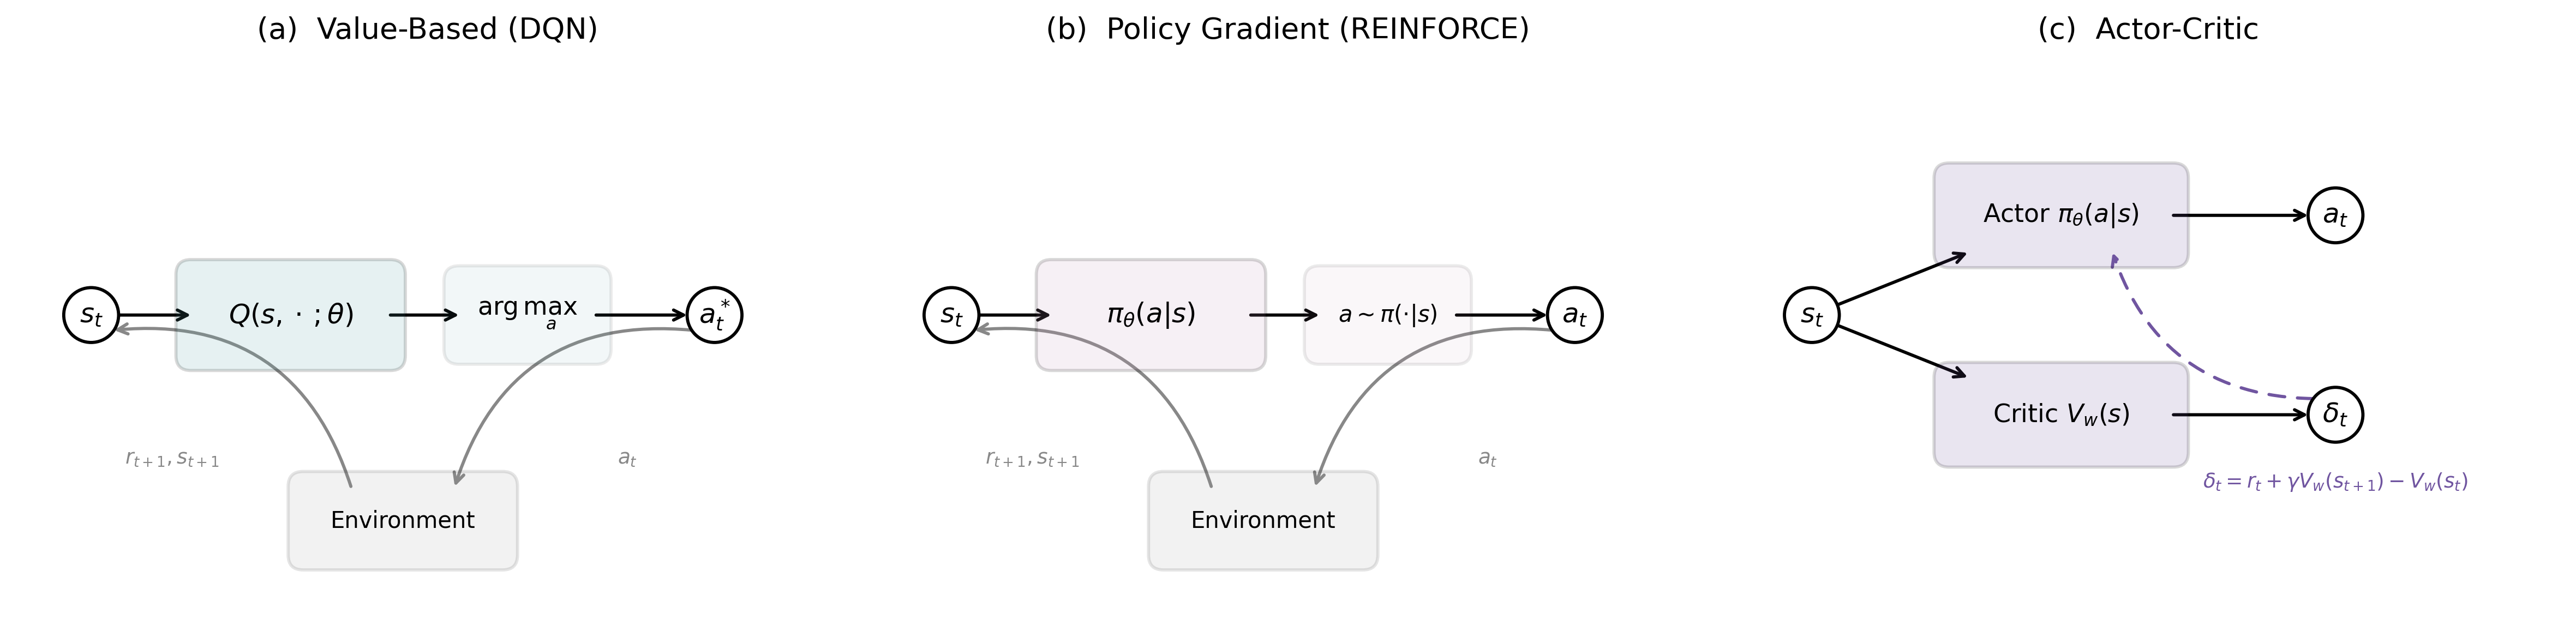
\includegraphics[width=\textwidth]{../ch02_rl_algorithms/sims/algorithm_architectures.png}
\caption{Architecture comparison of the three fundamental algorithm families. (a) DQN maps states to Q-values for all actions, selecting the argmax. (b) REINFORCE maps states to a probability distribution over actions, then samples. (c) Actor-Critic maintains separate policy and value networks; the critic's TD error $\delta_t$ provides a low-variance learning signal to the actor.}
\label{fig:algorithm_architectures}
\end{figure}

\FloatBarrier
\subsubsection{Control as Probabilistic Inference}
\label{sec:control_inference}

The \emph{control-as-inference} framework \citep{Todorov2006, Kappen2011, Ziebart2010, Levine2018} recasts the preceding algorithms as instances of probabilistic inference (computation, not statistical inference) in a single graphical model.\footnote{The framework is a mathematical language, much like random utility in econometrics, that reveals structural connections rather than deriving algorithms from first principles.} The payoff is that every advance in approximate inference (variational methods, message passing, amortized inference) becomes a candidate RL algorithm, and the forward problem (finding the optimal policy given rewards) and the inverse problem (recovering rewards from observed behavior) become two queries in the same model. The construction introduces a binary ``optimality'' variable $\mathcal{O}_t \in \{0,1\}$ at each time step, appended to the standard state-action-dynamics chain (Figure~\ref{fig:control_inference_dag}). The distribution over this variable is defined as
\begin{equation}
P(\mathcal{O}_t = 1 \mid s_t, a_t) = \exp(r(s_t, a_t)/\tau)
\label{eq:optimality_variable}
\end{equation}
where $\tau > 0$ is a temperature parameter and rewards satisfy $r \leq 0$.\footnote{The non-positive reward assumption ensures $\exp(r/\tau) \in (0,1]$. Any bounded reward can be shifted to satisfy this without changing the optimal policy. Alternatively, the optimality variable can be replaced by an undirected potential $\Phi(s_t, a_t) = \exp(r(s_t,a_t)/\tau)$, yielding a conditional random field formulation that removes this restriction \citep{Ziebart2010}.} This is a modeling assumption, not a derivation from first principles; the exponential form is chosen so the resulting posterior matches entropy-regularized RL.

\begin{figure}[t]
\centering
\begin{tikzpicture}[
    state/.style={circle, draw, minimum size=8mm, inner sep=0pt, fill=rlblue!10, draw=rlblue!60, line width=0.5pt, font=\small},
    action/.style={circle, draw, minimum size=8mm, inner sep=0pt, fill=rlgray!15, line width=0.5pt, font=\small},
    opt/.style={circle, draw, minimum size=8mm, inner sep=0pt, fill=rlorange!20, draw=rlorange!70, line width=0.5pt, font=\small},
    arr/.style={-{Stealth[length=2mm]}, line width=0.5pt},
    dotsty/.style={font=\large, rlgray},
]
% States (offset left within each time step)
\node[state] (s1) at (-0.7, 0) {$s_1$};
\node[state] (s2) at (2.8, 0) {$s_2$};
\node[state] (s3) at (6.3, 0) {$s_3$};
\node[dotsty] at (8.8, 0) {$\cdots$};
% Actions (offset right within each time step)
\node[action] (a1) at (0.7, 1.5) {$a_1$};
\node[action] (a2) at (4.2, 1.5) {$a_2$};
\node[action] (a3) at (7.7, 1.5) {$a_3$};
% Optimality variables (centered above each pair)
\node[opt] (o1) at (0, 3) {$\mathcal{O}_1$};
\node[opt] (o2) at (3.5, 3) {$\mathcal{O}_2$};
\node[opt] (o3) at (7.0, 3) {$\mathcal{O}_3$};
% Dynamics: (s_t, a_t) -> s_{t+1}
\draw[arr] (s1) -- (s2);
\draw[arr] (a1) -- (s2);
\draw[arr] (s2) -- (s3);
\draw[arr] (a2) -- (s3);
\draw[arr] (s3) -- (8.3, 0);
\draw[arr] (a3) -- (8.3, 0);
% Optimality: (s_t, a_t) -> O_t (no crossing)
\draw[arr] (s1) -- (o1);
\draw[arr] (a1) -- (o1);
\draw[arr] (s2) -- (o2);
\draw[arr] (a2) -- (o2);
\draw[arr] (s3) -- (o3);
\draw[arr] (a3) -- (o3);
\end{tikzpicture}
\caption{The control-as-inference graphical model. States $s_t$ and actions $a_t$ jointly determine the next state $s_{t+1}$ (dynamics) and the optimality variable $\mathcal{O}_t$ (reward signal). Optimality nodes $\mathcal{O}_t$ are observed as $\mathcal{O}_t = 1$; the posterior over actions $P(a_t \mid s_t, \mathcal{O}_{t:T} = 1)$ yields the optimal policy.}
\label{fig:control_inference_dag}
\end{figure}

The RL problem becomes a probabilistic inference query. Given that all future time steps are optimal ($\mathcal{O}_{t:T} = 1$), what is $P(a_t \mid s_t, \mathcal{O}_{t:T} = 1)$? Define backward messages $\beta_t(s, a) = P(\mathcal{O}_{t:T} = 1 \mid s_t = s,\, a_t = a)$, the probability that everything from $t$ onward is optimal given the agent is in state $s$ taking action $a$. These are computed by backward recursion:
\begin{align}
\beta_T(s, a) &= \exp(r(s, a)/\tau) \label{eq:beta_base} \\
\beta_t(s, a) &= \exp(r(s, a)/\tau) \sum_{s'} P(s'|s,a) \, \beta_{t+1}(s') \quad (t < T) \label{eq:beta_recursion}
\end{align}
where $\beta_{t+1}(s') \propto \sum_{a'} \beta_{t+1}(s', a')$ marginalizes over future actions under a uniform prior. By Bayes' rule, the posterior over actions is $P(a_t \mid s_t, \mathcal{O}_{t:T} = 1) = \beta_t(s_t, a_t) \,/\, \sum_{a'} \beta_t(s_t, a')$. Defining $Q(s,a) = \tau \log \beta_t(s,a)$, so that backward messages in log-space correspond to soft value functions, and $V(s) = \tau \log \sum_a \exp(Q(s,a)/\tau)$\footnote{Since $\beta_t(s) \propto \sum_a \beta_t(s,a) = \sum_a \exp(Q(s,a)/\tau)$, we have $V(s) = \tau \log \sum_a \exp(Q(s,a)/\tau)$.}, the posterior becomes $\pi(a \mid s) = \exp\bigl((Q(s,a) - V(s))/\tau\bigr)$, the softmax over Q-values.

Exact inference in this graphical model under stochastic dynamics produces risk-seeking policies. The backup becomes $Q(s,a) = r(s,a) + \tau \log \mathbb{E}_{s'}[\exp(V(s')/\tau)]$, which overweights unlikely favorable transitions because the agent implicitly assumes it can influence the dynamics.\footnote{Under exact inference, the posterior dynamics $P(s'|s,a,\mathcal{O}_{1:T}=1)$ differ from the true dynamics $P(s'|s,a)$, biasing the inferred transitions toward favorable outcomes. The log-expectation-of-exponentials exceeds the expectation by Jensen's inequality. This optimism is an artifact of exact inference in the model, not a feature.} The framework corrects this by applying structured variational inference, restricting the variational family to distributions that match the true dynamics $P(s'|s,a)$. This yields the soft Bellman equations
\begin{align}
Q(s,a) &= r(s,a) + \gamma \, \mathbb{E}_{s' \sim P}[V(s')] \label{eq:soft_bellman_q} \\
V(s) &= \tau \log \sum_{a \in \mathcal{A}} \exp\!\left(\frac{Q(s,a)}{\tau}\right) \label{eq:soft_bellman_v}
\end{align}
with the optimal policy given by $\pi(a \mid s) = \exp\bigl((Q(s,a) - V(s))/\tau\bigr)$. The operator $\mathcal{T}^{\mathrm{soft}}$ defined by Equations~\eqref{eq:soft_bellman_q}--\eqref{eq:soft_bellman_v} is a $\gamma$-contraction in $\|\cdot\|_\infty$, with the same convergence rate as the standard Bellman operator.\footnote{The proof follows from the log-sum-exp being 1-Lipschitz in the sup norm; see \citet{Haarnoja2017}, Theorem~1.} As $\tau \to 0$, the log-sum-exp converges to the hard maximum and the soft Bellman equations reduce to the standard Bellman optimality equations. The value function in Equation~\eqref{eq:soft_bellman_v} is identical to McFadden's social surplus function from discrete choice theory \citep{McFadden1978}, completing the connection noted in the preceding subsection.

Classical RL already employs exploration strategies ($\varepsilon$-greedy, UCB), but these are designed separately from the optimization objective. In the probabilistic framework, the objective itself maximizes expected reward and policy entropy simultaneously.\footnote{The max-ent objective is $\max_\pi \sum_t \mathbb{E}[r(s_t,a_t) + \tau \mathcal{H}(\pi(\cdot|s_t))]$. This equals the evidence lower bound (ELBO) of the graphical model, a quantity from variational inference that lower-bounds the log-likelihood of the observed optimality evidence $\log P(\mathcal{O}_{1:T} = 1)$. Maximizing the ELBO with respect to the policy is equivalent to finding the best approximation to the true posterior, measured by KL divergence; see \citet{BleiKucukelbirMcAuliffe2017} for a review of variational inference.} The Q-function, the value function, and the exploration behavior are all derived from a single objective. Different approximation strategies applied to this single model recover familiar algorithms. When the backward messages in Equations~\eqref{eq:beta_base}--\eqref{eq:beta_recursion} are computed exactly in the tabular setting, the result is soft value iteration. Estimating the ELBO gradient via the likelihood ratio trick yields max-ent policy gradients, identical to REINFORCE with $-\tau \log \pi(a_t|s_t)$ added to the reward at each step. Fitting parameterized $Q_\phi$ and $V_\psi$ networks to approximate the backward messages gives Soft Actor-Critic \citep{Haarnoja2018}. Fitting $Q_\phi$ alone and extracting the policy implicitly via the softmax gives soft Q-learning \citep{Haarnoja2017}. Trust-region methods such as TRPO and PPO do not optimize the max-ent objective, but each policy update step solves a max-ent subproblem with the old policy as prior, so the per-step structure mirrors the framework even though the global target remains standard reward maximization \citep{Schulman2015, Schulman2017}. Hard-max algorithms (Q-learning, DQN, standard policy gradient) are not direct instances of the framework; they are recovered in the zero-temperature limit $\tau \to 0$, where the softmax collapses to the argmax. Reading the graphical model in the reverse direction, treating the reward as the unknown and observed behavior as evidence of optimality, yields maximum entropy inverse reinforcement learning \citep{Ziebart2008}, connecting to the structural estimation methods discussed in Section~\ref{section:rl_econ_models}.

The framework has practical limitations. The converged fixed point is $Q^*_{\mathrm{soft}}$, not $Q^*$; at any $\tau > 0$, the policy is suboptimal for the original reward-maximization objective. The entropy bonus produces undirected exploration, spreading probability mass rather than targeting uncertain states. In safety-critical environments, the objective assigns nonzero probability to catastrophic actions. The practical benefits of the probabilistic perspective, including robustness to model perturbations and smooth optimization landscapes, are most apparent in continuous-control and robotics settings. In perfectly simulated environments with exact rewards (Atari, Go), the hard-max algorithms that dominate those domains do not require this probabilistic formulation, as the following subsection illustrates.

\subsubsection{AlphaGo Zero (2017)}
\label{subsubsec:alphago_zero}

The game of Go has approximately $10^{170}$ legal positions and a branching factor of roughly 250, far beyond the reach of brute-force search. Hand-crafted evaluation functions, which had succeeded in chess, failed here because positional concepts like influence, territory, and group viability are holistic and contextual. Monte Carlo tree search (MCTS) had achieved amateur-level play by using random simulations to estimate position values, but progress had stalled below professional strength. \citet{Silver2016} broke through by combining supervised learning from 30 million human expert positions, reinforcement learning via self-play, and MCTS with learned value and policy networks; the resulting system defeated Lee Sedol four games to one in March 2016. A year later, \citet{Silver2017} showed that none of the human data was necessary.

AlphaGo Zero uses a single convolutional neural network $f_\theta(s) = (\mathbf{p}, v)$ that takes a board position $s$ and outputs both a policy vector $\mathbf{p}$ over legal moves and a scalar value $v$ estimating the probability of winning. The input representation consists of 17 binary planes on the $19 \times 19$ board encoding the raw game state without hand-crafted features.\footnote{Eight planes for Black's stone positions over the last eight moves, eight for White's, and one indicating which color plays next. The history planes allow the network to detect ko situations and infer the trajectory of play.} The architecture uses residual blocks,\footnote{A residual block computes $\mathbf{x} + g(\mathbf{x})$ rather than just $g(\mathbf{x})$, where $g$ is a learned transformation. The skip connection allows gradients to flow through very deep networks without vanishing. AlphaGo Zero's 40-block architecture has 79 parameterized layers.} which allow training of very deep networks.

During play, each move is selected by running MCTS, which conducts 1,600 simulated games from the current position to estimate move quality. Each simulation proceeds in four phases, illustrated in Figure~\ref{fig:mcts_phases}. In the selection phase, the algorithm starts from the current position and traverses the partially built search tree by choosing at each node the action that maximizes $Q(s,a) + c_{\text{puct}} \cdot P(s,a) \cdot \sqrt{\sum_b N(s,b)} \,/\, (1 + N(s,a))$, where $Q(s,a)$ is the current average value of action $a$, $P(s,a)$ is the prior probability from the neural network, and $N(s,a)$ is the visit count.\footnote{The constant $c_{\text{puct}}$ controls exploration. Actions visited often have well-estimated $Q$ values but a shrinking exploration bonus; rarely visited actions have uncertain values but a large bonus. This is a continuous analogue of the upper confidence bound (UCB) strategy from bandit theory.} In the expansion and evaluation phase, when the traversal reaches a position not yet in the tree, the neural network evaluates it in a single forward pass, producing a policy vector $\mathbf{p}$ and a value estimate $v$; the policy initializes prior probabilities $P(s',a) = p_a$ for each child edge. In the backup phase, the value $v$ propagates back up the traversed path, incrementing each edge's visit count $N(s,a)$ and updating its mean value $Q(s,a)$. After all 1,600 simulations, the algorithm selects the move with the highest visit count at the root.

\begin{figure}[t]
\centering
\begin{tikzpicture}[
    nd/.style={circle, draw, minimum size=5mm, inner sep=0pt, fill=rlgray!12, line width=0.4pt},
    sel/.style={circle, draw, minimum size=5mm, inner sep=0pt, fill=rlblue!15, draw=rlblue!60, line width=0.7pt},
    newnd/.style={circle, draw, dashed, minimum size=5mm, inner sep=0pt, fill=rlgreen!10, draw=rlgreen!50!black, line width=0.7pt},
    edg/.style={-, rlgray!40, line width=0.3pt},
    sedg/.style={-, rlblue!60, line width=0.9pt},
    bedg/.style={-{Stealth[length=1.8mm]}, rlred!60, line width=0.7pt},
    phaselabel/.style={font=\footnotesize, anchor=north},
]
% ---- Panel 1: Selection ----
\begin{scope}[shift={(0,0)}]
    \node[sel] (r1) at (0,0) {};
    \node[nd] (a1) at (-0.9,-1.1) {};
    \node[sel] (b1) at (0.9,-1.1) {};
    \node[nd] (c1) at (-1.4,-2.2) {};
    \node[nd] (d1) at (-0.4,-2.2) {};
    \node[sel] (e1) at (0.5,-2.2) {};
    \node[nd] (f1) at (1.3,-2.2) {};
    \draw[edg] (r1) -- (a1);
    \draw[sedg] (r1) -- (b1);
    \draw[edg] (a1) -- (c1);
    \draw[edg] (a1) -- (d1);
    \draw[sedg] (b1) -- (e1);
    \draw[edg] (b1) -- (f1);
    \node[phaselabel] at (0,-2.9) {(a) Selection};
\end{scope}
% ---- Panel 2: Expansion ----
\begin{scope}[shift={(3.8,0)}]
    \node[nd] (r2) at (0,0) {};
    \node[nd] (a2) at (-0.9,-1.1) {};
    \node[nd] (b2) at (0.9,-1.1) {};
    \node[nd] (c2) at (-1.4,-2.2) {};
    \node[nd] (d2) at (-0.4,-2.2) {};
    \node[nd] (e2) at (0.5,-2.2) {};
    \node[nd] (f2) at (1.3,-2.2) {};
    \node[newnd] (g2) at (0.5,-3.3) {};
    \draw[edg] (r2) -- (a2);
    \draw[edg] (r2) -- (b2);
    \draw[edg] (a2) -- (c2);
    \draw[edg] (a2) -- (d2);
    \draw[edg] (b2) -- (e2);
    \draw[edg] (b2) -- (f2);
    \draw[-, rlblue!60, dashed, line width=0.7pt] (e2) -- (g2);
    \node[phaselabel] at (0,-3.8) {(b) Expansion};
\end{scope}
% ---- Panel 3: Evaluation ----
\begin{scope}[shift={(7.6,0)}]
    \node[nd] (r3) at (0,0) {};
    \node[nd] (a3) at (-0.9,-1.1) {};
    \node[nd] (b3) at (0.9,-1.1) {};
    \node[nd] (c3) at (-1.4,-2.2) {};
    \node[nd] (d3) at (-0.4,-2.2) {};
    \node[nd] (e3) at (0.5,-2.2) {};
    \node[nd] (f3) at (1.3,-2.2) {};
    \node[newnd] (g3) at (0.5,-3.3) {};
    \draw[edg] (r3) -- (a3);
    \draw[edg] (r3) -- (b3);
    \draw[edg] (a3) -- (c3);
    \draw[edg] (a3) -- (d3);
    \draw[edg] (b3) -- (e3);
    \draw[edg] (b3) -- (f3);
    \draw[edg] (e3) -- (g3);
    \node[draw, rounded corners=2pt, fill=rlorange!12, font=\scriptsize, inner sep=3pt, draw=rlorange!60, line width=0.5pt] (nn3) at (-0.9,-3.3) {$f_\theta$};
    \draw[-{Stealth[length=1.8mm]}, rlorange!60, line width=0.6pt] (nn3) -- (g3) node[midway, above, font=\tiny, yshift=1pt] {$(\mathbf{p}, v)$};
    \node[phaselabel] at (0,-3.8) {(c) Evaluation};
\end{scope}
% ---- Panel 4: Backup ----
\begin{scope}[shift={(11.4,0)}]
    \node[sel] (r4) at (0,0) {};
    \node[nd] (a4) at (-0.9,-1.1) {};
    \node[sel] (b4) at (0.9,-1.1) {};
    \node[nd] (c4) at (-1.4,-2.2) {};
    \node[nd] (d4) at (-0.4,-2.2) {};
    \node[sel] (e4) at (0.5,-2.2) {};
    \node[nd] (f4) at (1.3,-2.2) {};
    \node[newnd] (g4) at (0.5,-3.3) {};
    \draw[edg] (r4) -- (a4);
    \draw[edg] (r4) -- (b4);
    \draw[edg] (a4) -- (c4);
    \draw[edg] (a4) -- (d4);
    \draw[edg] (b4) -- (e4);
    \draw[edg] (b4) -- (f4);
    \draw[edg] (e4) -- (g4);
    \draw[bedg] ([xshift=2pt]g4.north) -- ([xshift=2pt]e4.south);
    \draw[bedg] ([xshift=2pt]e4.north) -- ([xshift=-2pt]b4.south);
    \draw[bedg] ([xshift=2pt]b4.north) -- ([xshift=2pt]r4.south);
    \node[font=\tiny, rlred!60, anchor=west] at (0.85,-2.75) {$v$};
    \node[phaselabel] at (0,-3.8) {(d) Backup};
\end{scope}
\end{tikzpicture}
\caption{The four phases of a single MCTS simulation in AlphaGo Zero. (a) Selection traverses the tree from the root, choosing at each node the action maximizing a UCB-like score balancing exploitation ($Q$) and exploration ($P/N$). (b) Expansion adds a new leaf node when the traversal reaches an unexplored position. (c) The neural network $f_\theta$ evaluates the new position, producing move priors $\mathbf{p}$ and a value estimate $v$. (d) Backup propagates $v$ along the traversed path, updating mean values $Q(s,a)$ and visit counts $N(s,a)$ at each edge.}
\label{fig:mcts_phases}
\end{figure}

The training loop generates self-play games. At each board position $s_t$ during a game, the program runs MCTS to produce improved move probabilities $\boldsymbol{\pi}_t$, where $\pi_t(a) \propto N(s_t, a)^{1/\tau}$ and $\tau$ is a temperature parameter controlling exploration.\footnote{Early in the game ($t \leq 30$), $\tau = 1$ so moves are sampled proportionally to visit counts, encouraging diverse openings. Later, $\tau \to 0$ and the most-visited move is selected deterministically. Dirichlet noise is also added to root priors, $P(s,a) = (1 - \varepsilon)p_a + \varepsilon \eta_a$ with $\eta \sim \text{Dir}(0.03)$, ensuring all legal moves can be explored despite strong network priors.} A move $a_t$ is sampled from $\boldsymbol{\pi}_t$ and played. At game end, the outcome $z \in \{-1, +1\}$ is recorded. Each position becomes a training triple $(s_t, \boldsymbol{\pi}_t, z)$, and the network parameters are updated to minimize
\begin{equation}
\ell(\theta) = (z - v)^2 - \boldsymbol{\pi}^\top \log \mathbf{p} + c \|\theta\|^2
\end{equation}
where the first term is a value prediction loss, the second is a policy cross-entropy loss,\footnote{The cross-entropy loss $-\boldsymbol{\pi}^\top \log \mathbf{p}$ measures how well the predicted distribution $\mathbf{p}$ matches the target $\boldsymbol{\pi}$; it equals zero when the distributions are identical.} and the third is $L_2$ regularization.\footnote{$L_2$ regularization penalizes the squared magnitude of parameters, $c\|\theta\|^2$, analogous to ridge regression in econometrics.} The key mechanism is a virtuous cycle. MCTS serves as a policy improvement operator, since the search probabilities $\boldsymbol{\pi}$ are stronger than the raw network outputs $\mathbf{p}$. Training the network to match $\boldsymbol{\pi}$ distills the search improvements back into the network, and the improved network in turn produces better MCTS. After 72 hours of self-play on 4 TPUs, AlphaGo Zero surpassed all previous versions, including the one that defeated Lee Sedol, and discovered novel strategies not previously seen in human play.\footnote{The system that defeated Lee Sedol in March 2016 used fixed network weights throughout the match; no parameter updates occurred between or during games. This illustrates the training-execution distinction (Section~\ref{section:language}): the months of self-play constituted the training phase, while the five-game match was purely execution.}

Go was well-suited to this architecture. Its fixed $19 \times 19$ board maps naturally to convolutional networks, its perfect information and deterministic transitions make MCTS's tree structure exact, and the binary game outcome provides an unambiguous training signal. \citet{Igami2020} interprets the architecture in econometric terms, where the policy network is a conditional choice probability (CCP) estimator, the value network is a conditional value function (CVF) estimator, and the system performs CCP estimation and forward simulation jointly, connecting to the approach of \citet{HotzMiller1993} in dynamic discrete choice.


\subsubsection{Decision Transformers (2021)}
\label{subsubsec:decision_transformers}

\citet{Chen2021DT} proposed replacing Bellman backups with autoregressive
sequence modeling. The Decision Transformer conditions a causal GPT-style
Transformer on trajectories $\tau = (\hat{R}_1, s_1, a_1, \hat{R}_2, s_2,
a_2, \ldots)$, where $\hat{R}_t$ is the \emph{return-to-go} (desired future
cumulative reward). At test time, conditioning on a high target return
extracts a high-performing policy without any temporal-difference learning.
\citet{Janner2021TT} extended this to the Trajectory Transformer, modeling
entire trajectories as flat token sequences with continuous dimensions
discretized into bins, enabling planning via beam search over trajectories.

The approach has fundamental limitations that Bellman-based methods do not
share. \citet{Brandfonbrener2022} proved that return-conditioned supervised
learning (RCSL) recovers optimal policies only under assumptions strictly
stronger than those needed for dynamic programming: near-deterministic
dynamics, expert data coverage, and a unique mapping from returns to optimal
actions. In stochastic environments, high returns may reflect environmental
luck rather than good decisions, causing RCSL to imitate lucky-but-suboptimal
trajectories. \citet{Paster2022} demonstrated this concretely: in a simple
gambling MDP, the Decision Transformer conditioned on high returns selects
risky gambles over the optimal safe action, even with infinite
data.\footnote{\citet{Emmons2022} showed that a simple two-layer MLP matches
the Transformer architecture on D4RL benchmarks, suggesting the
autoregressive structure provides conditional density estimation rather than
temporal reasoning. The essential element is conditioning on the right outcome
variable, not the architecture.}

A second limitation is that RCSL cannot \emph{stitch} suboptimal trajectory
segments. If the dataset contains two trajectories that each visit a useful
intermediate state but from different starting points, Bellman-based methods
can compose the better segments by propagating values backward through the
shared state. Sequence models, which predict forward autoregressively, cannot
perform this backward composition.